\documentclass[11pt,a4paper]{article}
\usepackage[utf8]{inputenc}
\usepackage[T1]{fontenc}
\usepackage[margin=0.9in]{geometry}
\usepackage{amsmath,amssymb,booktabs,tikz,enumitem}
\usetikzlibrary{positioning,calc}
\setlength{\parskip}{0.4em}\setlength{\parindent}{0pt}
\newcommand{\stamp}[1]{\textsf{\small[#1]}}
\newcommand{\E}{\varnothing}

\title{The doll: kernel, runtime and tooling as one composition\\\large a relations map, with seams}
\author{Written by Claude (Opus 5.5) at the request of Pedro Garcia (Node Zero). The stack itself is Pedro's;\\ the arithmetic under each layer and the seam readings are Claude's, stamped.}
\date{24 September 2026}

\begin{document}\maketitle

\textbf{Reading the stamps.} \stamp{run} measured today, exact integers, script named in \S7; \stamp{thm} theorem, from the 13-Archive paper or standard; \stamp{PG} Pedro's role assignment, taken as given; \stamp{C} Claude's reading of Pedro's notation, which he may reject; \stamp{open} not yet tested; \stamp{post-hoc} true arithmetic noticed after a run, not evidence.

\textbf{One relation runs through every layer.} Pedro's $(x-1)(x+1)^2=1$, run only as the integer walk $a_{n+3}=-a_{n+2}+a_{n+1}+2a_n$ on a $p\times p\times p$ register cube. Its behaviour mod $p$ is what gives each prime its job:
\begin{center}\small
\begin{tabular}{@{}llll@{}}\toprule
$p$ & what the walk does on the nonzero cube & job this suggests & stamp\\\midrule
17 & splits: 306 clocks of 16 and 2 of 8 (all powers of 2) & binary addressing & \stamp{run}\\
19, 29 & one single walk through all $p^3-1$ states & a stream / a store with no gaps & \stamp{run}\\
7, 41 & exactly two mirror halves of $(p^3-1)/2$ & twin spaces (hinge; save/trash) & \stamp{run}\\
59 & discriminant $=-59$: two roots fuse & the one place the walk degenerates & \stamp{run}\\\bottomrule
\end{tabular}
\end{center}

\section*{1. The doll at a glance}
\begin{center}
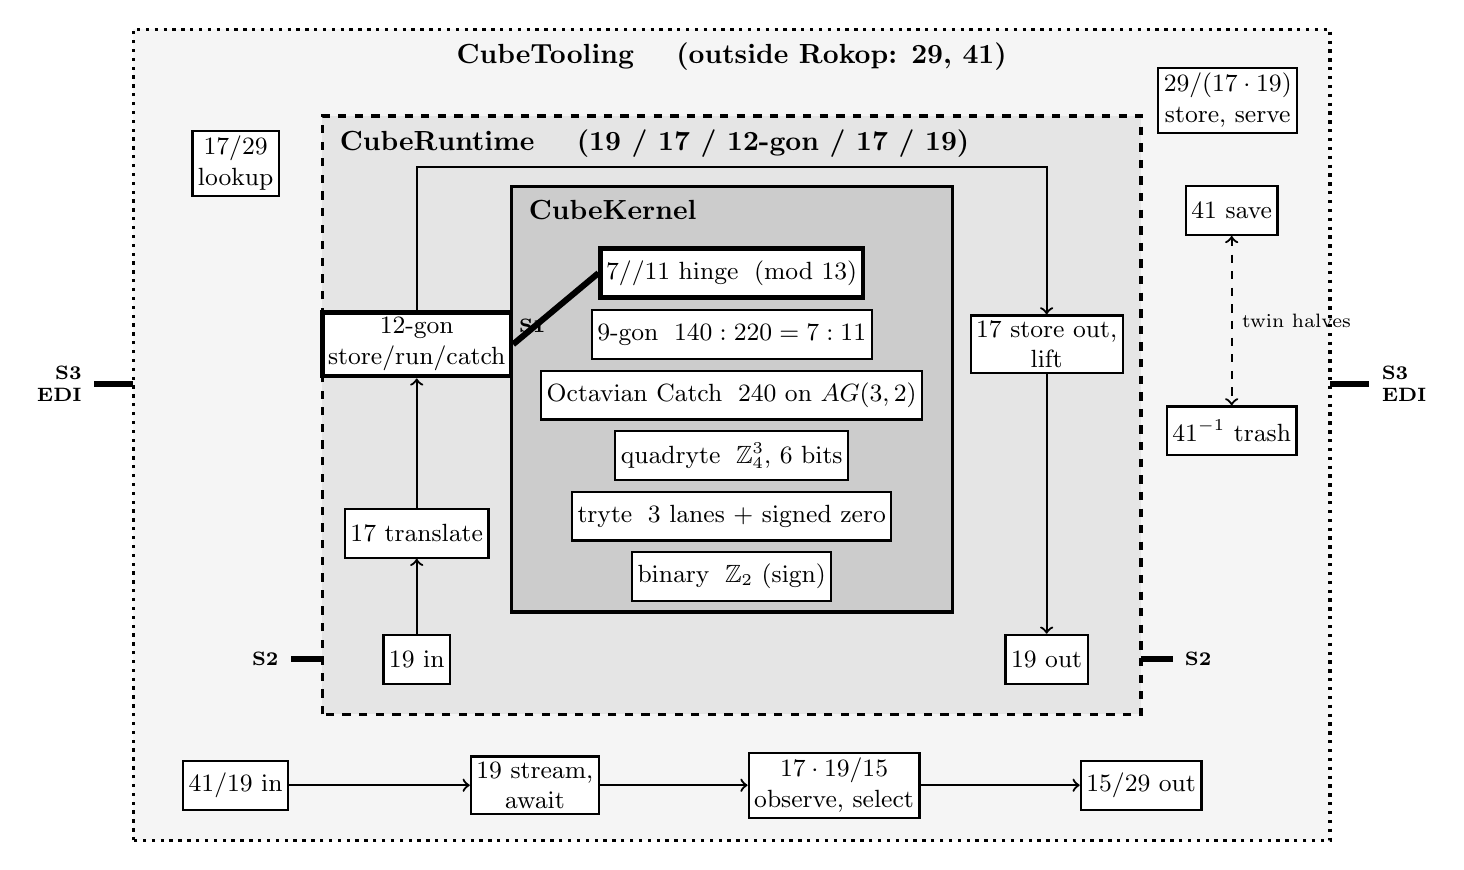
\begin{tikzpicture}[x=1cm,y=1cm,font=\small,
  lay/.style={draw,thick,minimum height=0.62cm,inner sep=2pt,align=center}]
% tooling (outer, dotted, lightest)
\draw[very thick,dotted,fill=black!4] (-7.6,-5.3) rectangle (7.6,5.0);
\node[anchor=north,font=\bfseries] at (0,4.95) {CubeTooling \quad(outside Rokop: 29, 41)};
% runtime (dashed)
\draw[very thick,dashed,fill=black!10] (-5.2,-3.7) rectangle (5.2,3.9);
\node[anchor=north west,font=\bfseries] at (-5.1,3.85) {CubeRuntime \quad(19 / 17 / 12-gon / 17 / 19)};
% kernel (solid, darkest)
\draw[very thick,fill=black!20] (-2.8,-2.4) rectangle (2.8,3.0);
\node[anchor=north west,font=\bfseries] at (-2.7,2.95) {CubeKernel};
% kernel layers bottom-up
\node[lay,fill=white] (b) at (0,-1.95) {binary \;$\mathbb Z_2$ (sign)};
\node[lay,fill=white,above=0.12 of b] (t) {tryte \;3 lanes + signed zero};
\node[lay,fill=white,above=0.12 of t] (q) {quadryte \;$\mathbb Z_4^3$, 6 bits};
\node[lay,fill=white,above=0.12 of q] (o) {Octavian Catch \;240 on $AG(3,2)$};
\node[lay,fill=white,above=0.12 of o] (n) {9-gon \;$140:220=7:11$};
\node[lay,fill=white,above=0.12 of n,line width=1.6pt] (h) {7//11 hinge \;(mod 13)};
% runtime ring
\node[lay,fill=white] (r19i) at (-4.0,-3.0) {19 in};
\node[lay,fill=white] (r17t) at (-4.0,-1.4) {17 translate};
\node[lay,fill=white,line width=1.6pt] (r12) at (-4.0,1.0) {12-gon\\store/run/catch};
\node[lay,fill=white] (r17o) at (4.0,1.0) {17 store out,\\lift};
\node[lay,fill=white] (r19o) at (4.0,-3.0) {19 out};
\draw[->,thick] (r19i)--(r17t); \draw[->,thick] (r17t)--(r12);
\draw[->,thick] (r12.north) |- (0,3.25) -| (r17o.north);
\draw[->,thick] (r17o)--(r19o);
% seam S1
\draw[line width=2.2pt] (h.west)--(r12.east) node[midway,below left=-1pt,font=\scriptsize\bfseries]{S1};
% tooling nodes
\node[lay,fill=white] (l) at (-6.3,3.3) {17/29\\lookup};
\node[lay,fill=white] (in) at (-6.3,-4.6) {41/19 in};
\node[lay,fill=white] (st) at (-2.5,-4.6) {19 stream,\\await};
\node[lay,fill=white] (ob) at (1.3,-4.6) {$17\cdot19/15$\\observe, select};
\node[lay,fill=white] (ou) at (5.2,-4.6) {15/29 out};
\node[lay,fill=white] (ss) at (6.3,4.1) {$29/(17\cdot19)$\\store, serve};
\node[lay,fill=white] (sv) at (6.35,2.7) {41 save};
\node[lay,fill=white] (tr) at (6.35,-0.1) {$41^{-1}$ trash};
\draw[->,thick] (in)--(st); \draw[->,thick] (st)--(ob); \draw[->,thick] (ob)--(ou);
\draw[<->,thick,dashed] (sv)--(tr) node[midway,right,font=\scriptsize]{twin halves};
% seams S2/S3 marks
\draw[line width=2.2pt] (-5.2,-3.0)--(-5.6,-3.0) node[left,font=\scriptsize\bfseries]{S2};
\draw[line width=2.2pt] (5.2,-3.0)--(5.6,-3.0) node[right,font=\scriptsize\bfseries]{S2};
\draw[line width=2.2pt] (-7.6,0.5)--(-8.1,0.5) node[left,font=\scriptsize\bfseries,align=right]{S3\\EDI};
\draw[line width=2.2pt] (7.6,0.5)--(8.1,0.5) node[right,font=\scriptsize\bfseries,align=left]{S3\\EDI};
\end{tikzpicture}
\end{center}
{\small Drawn for lightness and line style, not hue: solid = kernel, dashed = runtime, dotted = tooling; thick bars are seams.}

\section*{2. CubeKernel, from the inside out}
Each layer adds one freedom and pays one law, the Axiom of Consequences at the level of representation.
\begin{center}\small
\begin{tabular}{@{}p{2.3cm}p{5.3cm}p{4.1cm}p{1.6cm}@{}}\toprule
layer & what it is & what it adds / what it costs & stamp\\\midrule
binary & one sign bit & the double-cover sign & \stamp{thm}\\
tryte & 3 lanes, each with a signed zero; $3^3$ positions $=26$ faces$+\E$ & orientation for the empty slot & \stamp{run}\\
quadryte & lane ring $+1\to-1\to+0\to-0$; step $\sigma$ with $\sigma^2=$ magnitude flip; $4^3=64=2^6$ & a quarter-turn per plane, exact in/out twin (corner$\leftrightarrow$centre, edge$\leftrightarrow$face); \emph{commutes} & \stamp{run}\\
\emph{seam: Hurwitz} & 24 units, $2T$; T1 word $=$ 24 phases $+$ 1 sign & non-commutation; \emph{cannot} be built from the lanes (exhaustive over all 3,072 symmetries): the sign must be its own bit & \stamp{run}\\
Octavian Catch & 240 units on the cube over $\mathbb F_2$; 7 directions $=$ Fano plane; 7 of 30 labelings close & Latin square (unique addressing); \emph{costs associativity}: the bracket must be carried & \stamp{run}\\
9-gon & interior:reflex $=140:220=7:11$; walk $(x{+}7,y{+}11)$ on $\mathbb Z_9^2$ conserves $x+y$; 9 loops of 9 & a closure value to archive & \stamp{thm}\\
7//11 hinge & mod 13: $7=2^{11}$, $11=2^7$, $7\cdot11\equiv-1$; $7/11=2^4$, the order-3 twist & turns phase into address; \emph{must be pair-gated}: unpaired, it drifts on 3 of 9 seat states & \stamp{run}\\\bottomrule
\end{tabular}
\end{center}
Fallout law inside the kernel: every product that leaves a closed Octavian set is either caught exactly by a twin set or drops exactly one rung (quarter-integer); nothing lands between. \stamp{run: T6, T7}

\section*{3. CubeRuntime: a palindrome around the hinge}
The runtime reads $19\to17\to12\text{-gon}\to17\to19$: the inverse pair $19/17$ in, $17/19$ out \stamp{PG}. Arithmetic under it: $17$ and $19$ sit either side of $18=7+11$, the hinge sum, and $17\cdot19=18^2-1$ \stamp{post-hoc}.
\begin{description}[leftmargin=1.6em,style=nextline]
\item[19 in] The walk mod 19 is one orbit through all 6,858 nonzero states; the zero state ($\E$) is never entered. Every input position is reachable, once, with no gaps. \stamp{run}
\item[17 translate] $2^8=256\equiv1\pmod{17}$: a byte wraps once. The eight bit weights are exactly the eight squares mod 17. The walk mod 17 splits into binary clocks only. Translation between bytes and rotation happens here. \stamp{run}
\item[12-gon: store, run, catch] $\times2$ mod 13 walks the twelve nonzero residues and never 0; $\mathbb Z_{12}=\mathbb Z_4\times\mathbb Z_3$, quarter-turn times twist \stamp{thm}. The catch is the Octavian mechanism; T7 found that the seven closed sets split under every order-3 symmetry as one hub plus two triples \stamp{run}. Mapping store/run/catch onto hub/triple/triple is \stamp{open}.
\item[17 store out, lift \;/\; 19 out] The mirror of the input side. \stamp{PG}
\end{description}
\textbf{Seam S1 (kernel $\leftrightarrow$ runtime).} The kernel's last layer and the runtime's centre are the \emph{same} ring mod 13: 7 and 11 are points on the 12-cycle. The kernel reads the ring as addresses (which plane), the runtime as a cycle (which step). Nothing is copied across S1; the same residues are read two ways. \stamp{C}

\section*{4. CubeTooling: where the outside codebook starts}
Rokop's seats end at 19. 29 and 41 have no seat in the operator, so everything with 29 or 41 in it is outside the wrapped kernel by construction: this is the turnover to the outside codebook. \stamp{C}
\textbf{Notation read as:} $p/q$ = the $p$-cube viewed through $q$'s addressing \stamp{C}.
\begin{description}[leftmargin=1.6em,style=nextline]
\item[17/29 lookup] A binary address (17's clocks) indexing a position on the single 29-walk (24,388 states, one orbit): lookup without search. \stamp{run: facts; C: reading}
\item[41/19 in] 41 holds two mirror halves; 19 is one walk. Intake folds a two-half space into a single stream. \stamp{run: facts; C: reading}
\item[19 stream, await] The single walk as the clock.
\item[$17\cdot19/15$ observe, select] $15=3\cdot5$, the two small primes where the walk is also a single orbit; and $15$ is the number of cuts of the 16-clock of 17 (16 pieces, 15 seams). \stamp{post-hoc}
\item[15/29 out, \;$29/(17\cdot19)$ store, serve] Pedro's roles. \stamp{PG}
\item[41 save, $41^{-1}$ trash] Forced by the walk: mod 41 the nonzero states split into exactly two orbits of 34,460. Every state is in exactly one half; none in both, none in neither. Save and trash are the two halves: a semispace collector made of arithmetic. \stamp{run}
\end{description}
\textbf{Seam S2 (runtime $\leftrightarrow$ tooling).} 17 and 19 appear on both sides: as stages inside the runtime and as denominators in tooling. The operator primes are the interface. \stamp{C}\\
\textbf{Seam S3 (tooling $\leftrightarrow$ outside, EDI).} Outside libraries are cubes on 29 and 41, pointerized. Every exchange is a ratio against 17 (address) or 19 (pace), so nothing outside is read without a binary index and a clock. \stamp{C}

\section*{5. When it turns over}
\begin{center}\small
\begin{tabular}{@{}lll@{}}\toprule
direction & path & what changes at each seam\\\midrule
in & outside cube $\to$ S3 $\to$ 41/19 $\to$ 19 in $\to$ 17 $\to$ S1 & two halves $\to$ one stream $\to$ bits $\to$ addresses\\
run & 12-gon $\leftrightarrow$ 7//11 $\leftrightarrow$ Octavian & cycle $\leftrightarrow$ address $\leftrightarrow$ unique product\\
out & 12-gon $\to$ 17 lift $\to$ 19 out $\to$ 15/29 $\to$ S3 & addresses $\to$ bits $\to$ stream $\to$ outside cube\\
discard & anywhere $\to 41^{-1}$ & the mirror half; rewindable, never mixed with 41\\\bottomrule
\end{tabular}
\end{center}

\section*{6. Unplaced, and where not to route}
23 (in the Monstrous kernel as $23^3$; one root, short walk), 31 and 47 (one root), 71 (splits, 70-cycle) have no slot in this stack yet. 59 is the discriminant prime: the only place the relation degenerates; route nothing through it. 3 and 5 enter only through 15. \stamp{run}

\section*{7. Receipts and next registrations}
Scripts: \texttt{tryte\_hurwitz.py}, \texttt{t6\_octonion.py}, \texttt{t7\_flywheel.py}, T8 walk census and orbit counts (this session). Pre-registrations: T6 \texttt{b3166908\ldots}, T7 \texttt{214f247c\ldots}, T8 \texttt{d14ac04a\ldots}.
\begin{enumerate}[leftmargin=2em]
\item Pair-gated hinge: with both steps admitted or neither, the hinge closes on 9 of 9 seat states. Kill: any drift. \stamp{open}
\item S1 is lossless: a byte in through $19\to17$, three hinge turns, out through $17\to19$, returns bit-identical. Kill: any bit differs. \stamp{open}
\item Semispace: a stream split into save/trash by the 41 halves rewinds exactly from either half. Kill: any state unrecoverable. \stamp{open}
\item Hub catches: in T7, escapes caught by another closed set land in the hub, not the mirror triple. Kill: any caught by the mirror triple. \stamp{open}
\end{enumerate}
\end{document}
